%-----------------------------------
% Define document and include general packages
%-----------------------------------
% Tabellen- und Abbildungsverzeichnis stehen normalerweise nicht im
% Inhaltsverzeichnis. Gleiches gilt für das Abkürzungsverzeichnis (siehe unten).
% Manche Dozenten bemängeln das. Die Optionen 'listof=totoc,bibliography=totoc'
% geben das Tabellen- und Abbildungsverzeichnis im Inhaltsverzeichnis (toc=Table
% of Content) aus.
% Da es aber verschiedene Regelungen je nach Dozent geben kann, werden hier
% beide Varianten dargestellt.
\documentclass[12pt,oneside,titlepage,listof=totoc,bibliography=totoc]{scrartcl}
% \documentclass[12pt,oneside,titlepage]{scrartcl}

%-----------------------------------
% Dokumentensprache
%-----------------------------------
%\def\FOMEN{}% Auskommentieren um die Dokumentensprache auf englisch zu ändern
\newif\ifde
\newif\ifen

%-----------------------------------
% Meta informationen
%-----------------------------------
%-----------------------------------
% Meta Informationen zur Arbeit
%-----------------------------------

% Autor
\newcommand{\myAutor}{Mads Fuchs, Nils Rüber, Janis Wiesen, Marlon Juntorius}

% Adresse
\newcommand{\myAdresse}{Heidestra\ss e 17 \\ \> \> \> 51147 Köln}

% Titel der Arbeit
\newcommand{\myTitel}{One-Klick Brand}

% Anzahl der Wörter
% \newcommand{\myAnzahlWoerter}{Anzahl Wörter Seminararbeit: 6413 | Anzahl Wörter im Programmcode: 425109}

% Anzahl der LinesOfCode
% \newcommand{\myLOC}{LOC: 62413}

% Betreuer
\newcommand{\myBetreuer}{Sandro Coletta}

% Lehrveranstaltung
\newcommand{\myLehrveranstaltung}{IT-Trends \& Innovation}

% Matrikelnummer
\newcommand{\myMatrikelNr}{675314, 674514, 670300, xxxxxx}

% Ort
\newcommand{\myOrt}{Bonn}

% Datum der Abgabe
\newcommand{\myAbgabeDatum}{12.01.2025}

% Semesterzahl
\newcommand{\mySemesterZahl}{5}

% Name der Hochschule
\newcommand{\myHochschulName}{FOM Hochschule für Oekonomie \& Management}

% Standort der Hochschule
\newcommand{\myHochschulStandort}{Bonn}

% Studiengang
\newcommand{\myStudiengang}{Wirtschaftsinformatik}

% Art der Arbeit
\newcommand{\myThesisArt}{Seminararbeit}


\ifdefined\FOMEN
%Englisch
\entrue
\usepackage[english]{babel}
\else
%Deutsch
\detrue
\usepackage[ngerman]{babel}
\fi


\newcommand{\langde}[1]{%
   \ifde\selectlanguage{ngerman}#1\fi}
\newcommand{\langen}[1]{%
   \ifen\selectlanguage{english}#1\fi}
\usepackage[utf8]{luainputenc}
\langde{\usepackage[babel,german=quotes]{csquotes}}
\langen{\usepackage[babel,english=british]{csquotes}}
\usepackage[T1]{fontenc}
\usepackage{fancyhdr}
\usepackage{fancybox}
\usepackage[a4paper, left=4cm, right=2cm, top=4cm, bottom=2cm]{geometry}
\usepackage{graphicx}
\usepackage{colortbl}
\usepackage[capposition=top]{floatrow}
\usepackage{array}
\usepackage{float}      %Positionierung von Abb. und Tabellen mit [H] erzwingen
\usepackage{footnote}
% Darstellung der Beschriftung von Tabellen und Abbildungen (Leitfaden S. 44)
% singlelinecheck=false: macht die Caption linksbündig (statt zentriert)
% labelfont auf fett: (Tabelle x.y:, Abbildung: x.y)
% font auf fett: eigentliche Bezeichnung der Abbildung oder Tabelle
% Fettschrift laut Leitfaden 2018 S. 45
\usepackage[singlelinecheck=false, labelfont=bf, font=bf]{caption}
\usepackage{caption}
\usepackage{enumitem}
\usepackage{amssymb}
% \usepackage{mathptmx}
\usepackage{minted} %Kann für schöneres Syntax Highlighting genutzt werden. ACHTUNG: Python muss installiert sein.
\usepackage[scaled=0.9]{helvet} % Behebt, zusammen mit Package courier, pixelige Überschriften. Ist, zusammen mit mathptx, dem times-Package vorzuziehen. Details: https://latex-kurs.de/fragen/schriftarten/Times_New_Roman.html
\usepackage{courier}
% \usepackage{amsmath}
\usepackage[table]{xcolor}
\usepackage{marvosym}			% Verwendung von Symbolen, z.B. perfektes Eurozeichen

\usepackage{scrhack} % behebt Warnungen und Fehlermeldungen

\renewcommand\familydefault{\sfdefault}
\usepackage{ragged2e}

% Mehrere Fussnoten nacheinander mit Komma separiert
\usepackage[hang,multiple]{footmisc}
\setlength{\footnotemargin}{1em}

% todo Aufgaben als Kommentare verfassen für verschiedene Editoren
\usepackage{todonotes}

% Verhindert, dass nur eine Zeile auf der nächsten Seite steht
\setlength{\marginparwidth}{2cm}
\usepackage[all]{nowidow}
\usepackage{appendix}

\addto\captionsngerman{% Replace "english" with the language you use
	\renewcommand{\contentsname}{Inhaltsverzeichnis}
	\renewcommand{\listfigurename}{Abbildungsverzeichnis}
	\renewcommand{\listtablename}{Tabellenverzeichnis}
	\renewcommand{\appendixname}{Anhang}
	\renewcommand{\figurename}{Abbildung}
	\renewcommand{\tablename}{Tabelle}
	\renewcommand{\appendixtocname}{Anhang}
	\appendixtitleon    % puts \appendixname before each appendix title
	%\renewcommand{\abbreHeadingName}{List of Abbreviations}
}

%-----------------------------------
% Farbdefinitionen
%-----------------------------------
\definecolor{darkblack}{rgb}{0,0,0}
\definecolor{dunkelgrau}{rgb}{0.8,0.8,0.8}
\definecolor{hellgrau}{rgb}{0.0,0.7,0.99}
\definecolor{mauve}{rgb}{0.58,0,0.82}
\definecolor{dkgreen}{rgb}{0,0.6,0}

%-----------------------------------
% Pakete für Tabellen
%-----------------------------------
\usepackage{epstopdf}
\usepackage{nicefrac} % Brüche
\usepackage{multirow}
\usepackage{rotating} % vertikal schreiben
\usepackage{mdwlist}
\usepackage{tabularx}% für Breitenangabe

%-----------------------------------
% sauber formatierter Quelltext
%-----------------------------------
\usepackage{listings, listings-rust}
% JavaScript als Sprache definieren:
\lstdefinelanguage{JavaScript}{
	keywords={break, super, case, extends, switch, catch, finally, for, const, function, try, continue, if, typeof, debugger, var, default, in, void, delete, instanceof, while, do, new, with, else, return, yield, enum, let, await},
	keywordstyle=\color{blue}\bfseries,
	ndkeywords={class, export, boolean, throw, implements, import, this, interface, package, private, protected, public, static},
	ndkeywordstyle=\color{darkgray}\bfseries,
	identifierstyle=\color{black},
	sensitive=false,
	comment=[l]{//},
	morecomment=[s]{/*}{*/},
	commentstyle=\color{purple}\ttfamily,
	stringstyle=\color{red}\ttfamily,
	morestring=[b]',
	morestring=[b]"
}

% \lstset{
% 	%language=JavaScript,
% 	numbers=left,
% 	numberstyle=\tiny,
% 	numbersep=5pt,
% 	breaklines=true,
% 	showstringspaces=false,
% 	frame=l ,
% 	xleftmargin=5pt,
% 	xrightmargin=5pt,
% 	basicstyle=\ttfamily\scriptsize,
% 	stepnumber=1,
% 	keywordstyle=\color{blue},          % keyword style
%   	commentstyle=\color{dkgreen},       % comment style
%   	stringstyle=\color{mauve}         % string literal style
% }


% Alternative Konfiguration für JavaScript Codehighlighting von ChatGPT
\lstset{
  language=JavaScript,                 	 % JavaScript-Syntax
  basicstyle=\ttfamily\small,          	 % Monospace-Schrift, klein
  keywordstyle=\color{blue},           	 % Keywords in Blau
  commentstyle=\color{green},         	 % Kommentare in Grün
  stringstyle=\color{red},            	 % Strings in Rot
  backgroundcolor=\color{lightgray}, 	 % Hintergrundfarbe
  numbers=left,                      	 % Zeilennummern links
  numberstyle=\tiny\color{gray},		 % Zeilennummern grau und klein
  frame=single,                          % Rahmen um den Code
  tabsize=2,                             % Tabulatorweite
  showstringspaces=false,                % Leerzeichen in Strings nicht anzeigen
  breaklines=true,                       % Lange Zeilen umbrechen
  morekeywords={useState,useEffect,props,import,export,from,return}, % Zusätzliche Schlüsselwörter
}


% \documentclass{article}
% \usepackage{xcolor}
% \usepackage{listings}


%-----------------------------------
%Literaturverzeichnis Einstellungen
%-----------------------------------

% Biblatex

\usepackage{url}
\urlstyle{same}

%%%% Neuer Leitfaden (2018)
\usepackage[
backend=biber,
style=ext-authoryear-ibid, % Auskommentieren und nächste Zeile einkommentieren, falls "Ebd." (ebenda) nicht für sich-wiederholende Fussnoten genutzt werden soll.
%style=ext-authoryear,
maxcitenames=3,	% mindestens 3 Namen ausgeben bevor et. al. kommt
maxbibnames=999,
mergedate=false,
date=iso,
seconds=true, %werden nicht verwendet, so werden aber Warnungen unterdrückt.
urldate=iso,
innamebeforetitle,
dashed=false,
autocite=footnote,
doi=false,
useprefix=true, % 'von' im Namen beachten (beim Anzeigen)
mincrossrefs = 1
]{biblatex}%iso dateformat für YYYY-MM-DD

%weitere Anpassungen für BibLaTex
\input{skripte/modsBiblatex2018}

%%%%% Alter Leitfaden. Ggf. Einkommentieren und Bereich hierüber auskommentieren
%\usepackage[
%backend=biber,
%style=numeric,
%citestyle=authoryear,
%url=false,
%isbn=false,
%notetype=footonly,
%hyperref=false,
%sortlocale=de]{biblatex}

%weitere Anpassungen für BibLaTex
%\input{skripte/modsBiblatex}

%%%% Ende Alter Leitfaden

%Bib-Datei einbinden
\addbibresource{literatur/literatur.bib}

% Zeilenabstand im Literaturverzeichnis ist Einzeilig
% siehe Leitfaden S. 14
\AtBeginBibliography{\singlespacing}

%-----------------------------------
% Silbentrennung
%-----------------------------------
\usepackage{hyphsubst}
\HyphSubstIfExists{ngerman-x-latest}{%
\HyphSubstLet{ngerman}{ngerman-x-latest}}{}

%-----------------------------------
% Pfad fuer Abbildungen
%-----------------------------------
\graphicspath{{./}{./figures/}}

%-----------------------------------
% Weitere Ebene einfügen
%-----------------------------------
\input{skripte/weitereEbene}

%-----------------------------------
% Paket für die Nutzung von Anhängen
%-----------------------------------
\usepackage{appendix}

%-----------------------------------
% Zeilenabstand 1,5-zeilig
%-----------------------------------
\usepackage{setspace}
\onehalfspacing

%-----------------------------------
% Absätze durch eine neue Zeile
%-----------------------------------
\setlength{\parindent}{0mm}
\setlength{\parskip}{0.8em plus 0.5em minus 0.3em}

\sloppy					%Abstände variieren
\pagestyle{headings}

%----------------------------------
% Präfix in das Abbildungs- und Tabellenverzeichnis aufnehmen, statt nur der Nummerierung (siehe Issue #206).
%----------------------------------
\KOMAoption{listof}{entryprefix} % Siehe KOMA-Script Doku v3.28 S.153
\BeforeStartingTOC[lof]{\renewcommand*\autodot{:}} % Für den Doppelpunkt hinter Präfix im Abbildungsverzeichnis
\BeforeStartingTOC[lot]{\renewcommand*\autodot{:}} % Für den Doppelpunkt hinter Präfix im Tabellenverzeichnis
%\BeforeStartingTOC[lol]{\renewcommand*\autodot{:}} % Für den Doppelpunkt hinter Präfix im Tabellenverzeichnis

%-----------------------------------
% PDF Meta Daten setzen
%-----------------------------------
\usepackage[hyperfootnotes=false]{hyperref} %hyperfootnotes=false deaktiviert die Verlinkung der Fußnote. Ansonsten inkompaibel zum Paket "footmisc"
% Behebt die falsche Darstellung der Lesezeichen in PDF-Dateien, welche eine Übersetzung besitzen
% siehe Issue 149
\makeatletter
\pdfstringdefDisableCommands{\let\selectlanguage\@gobble}
\makeatother

\hypersetup{
    pdfinfo={
        Title={\myTitel},
        Subject={\myStudiengang},
        Author={\myAutor},
        Build=1.1
    }
}

%-----------------------------------
% PlantUML
%-----------------------------------
%\usepackage{plantuml}

%-----------------------------------
% Umlaute in Code korrekt darstellen
% siehe auch: https://en.wikibooks.org/wiki/LaTeX/Source_Code_Listings
%-----------------------------------
\lstset{literate=
	{á}{{\'a}}1 {é}{{\'e}}1 {í}{{\'i}}1 {ó}{{\'o}}1 {ú}{{\'u}}1
	{Á}{{\'A}}1 {É}{{\'E}}1 {Í}{{\'I}}1 {Ó}{{\'O}}1 {Ú}{{\'U}}1
	{à}{{\`a}}1 {è}{{\`e}}1 {ì}{{\`i}}1 {ò}{{\`o}}1 {ù}{{\`u}}1
	{À}{{\`A}}1 {È}{{\'E}}1 {Ì}{{\`I}}1 {Ò}{{\`O}}1 {Ù}{{\`U}}1
	{ä}{{\"a}}1 {ë}{{\"e}}1 {ï}{{\"i}}1 {ö}{{\"o}}1 {ü}{{\"u}}1
	{Ä}{{\"A}}1 {Ë}{{\"E}}1 {Ï}{{\"I}}1 {Ö}{{\"O}}1 {Ü}{{\"U}}1
	{â}{{\^a}}1 {ê}{{\^e}}1 {î}{{\^i}}1 {ô}{{\^o}}1 {û}{{\^u}}1
	{Â}{{\^A}}1 {Ê}{{\^E}}1 {Î}{{\^I}}1 {Ô}{{\^O}}1 {Û}{{\^U}}1
	{œ}{{\oe}}1 {Œ}{{\OE}}1 {æ}{{\ae}}1 {Æ}{{\AE}}1 {ß}{{\ss}}1
	{ű}{{\H{u}}}1 {Ű}{{\H{U}}}1 {ő}{{\H{o}}}1 {Ő}{{\H{O}}}1
	{ç}{{\c c}}1 {Ç}{{\c C}}1 {ø}{{\o}}1 {å}{{\r a}}1 {Å}{{\r A}}1
	{€}{{\EUR}}1 {£}{{\pounds}}1 {„}{{\glqq{}}}1
}

%-----------------------------------
% Kopfbereich / Header definieren
%-----------------------------------
\pagestyle{fancy}

\fancyhf{}
% Seitenzahl oben, mittig, mit Strichen beidseits
% \fancyhead[C]{-\ \thepage\ -}

% Seitenzahl oben, mittig, entsprechend Leitfaden ohne Striche beidseits
\fancyhead[C]{\thepage}
%\fancyhead[L]{\leftmark}							% kein Footer vorhanden
% Waagerechte Linie unterhalb des Kopfbereiches anzeigen. Laut Leitfaden ist
% diese Linie nicht erforderlich. Ihre Breite kann daher auf 0pt gesetzt werden.
\renewcommand{\headrulewidth}{0.4pt}
%\renewcommand{\headrulewidth}{0pt}

%-----------------------------------
% Damit die hochgestellten Zahlen auch auf die Fußnote verlinkt sind (siehe Issue 169)
%-----------------------------------
\hypersetup{colorlinks=true, breaklinks=true, linkcolor=darkblack, citecolor=darkblack, menucolor=darkblack, urlcolor=darkblack, linktoc=all, bookmarksnumbered=false, pdfpagemode=UseOutlines, pdftoolbar=true}
\urlstyle{same}%gleiche Schriftart für den Link wie für den Text

%-----------------------------------
% Start the document here:
%-----------------------------------
\begin{document}

\pagenumbering{Roman}								% Seitennumerierung auf römisch umstellen
\newcolumntype{C}{>{\centering\arraybackslash}X}	% Neuer Tabellen-Spalten-Typ:
%Zentriert und umbrechbar

%-----------------------------------
% Textcommands
%-----------------------------------
%----------------------------------
%  TextCommands
%----------------------------------
%
%
%
%
%----------------------------------
%  common textCommands
%----------------------------------
% Information: OL bedeutet ohne Leerzeichen. Damit man dieses Command z. B. vor einem Komma oder vor einem anderen Zeichen verwenden kann. Dies ist ein Best-Practis von mir und hat sich sehr bewehrt.
% Allgemein hat es sich bewert alle Wörter die man häufig schreibt und wahrscheinlich falsch oder unterscheidlich schreibt, als Textcommand zu hinterlegen.
% 
%
%
%\renewcommand{\symheadingname}{\langde{Symbolverzeichnis}\langen{List of Symbols}}
\newcommand{\abbreHeadingName}{\langde{Abkürzungsverzeichnis}\langen{List of Abbreviations}}
\newcommand{\headingNameInternetSources}{\langde{Internetquellen}\langen{Internet sources}}
\newcommand{\AppendixName}{\langde{Anhang}\langen{Appendix}}
\newcommand{\vglf}{\langde{Vgl.}\langen{compare}}
\newcommand{\pagef}{\langde{S. }\langen{p. }}
\newcommand{\os}{\mbox{o. S}}
\newcommand{\ojol}{\mbox{o. J.}}
\newcommand{\oj}{\ojol\ }
\newcommand{\og}{\mbox{o. g.}\ }
\newcommand{\ua}{\mbox{u. a.}\ }
\newcommand{\dah}{\mbox{d. h.}\ }
\newcommand{\zbol}{\mbox{z. B.}}
\newcommand{\zb}{\zbol\ }
\newcommand{\uamol}{unter anderem}
\newcommand{\uam}{\uamol\ }
\newcommand{\uanol}{unter anderen}%mit Leerzeichen
\newcommand{\uan}{\uanol\ }%mit Leerzeichen
\newcommand{\abbol}{Ab"-bil"-dung}
\newcommand{\abb}{\abbol\ }
\newcommand{\tabol}{Tabelle}
\newcommand{\tab}{\tabol\ }
\newcommand{\ggfol}{ggf.}
\newcommand{\ggf}{\ggfol\ }
\newcommand{\unodol}{und/oder}
\newcommand{\unod}{\unodol\ }

%----------------------------------
% project individual textCommands
%----------------------------------
\newcommand{\lehol}{Lebensmitteleinzelhandel}%Beispiel eines langen Wortes
\newcommand{\leh}{\lehol\ }
\renewcommand{\figurename}{Abbildung}
\renewcommand{\listfigurename}{Abbildungsverzeichnis}
\renewcommand{\appendixtocname}{Anhang}
\newcommand{\vglfootcite}[2][]{\footcite[Vgl.][#1]{#2}}

%-----------------------------------
% Titlepage
%-----------------------------------
\begin{titlepage}
	\newgeometry{left=2cm, right=2cm, top=2cm, bottom=2cm}
	\begin{center}
    \includegraphics[width=2.3cm]{figures/fomLogo} \\
    \vspace{.5cm}
		\begin{Large}\textbf{\myHochschulName}\end{Large}\\
    \vspace{.5cm}
		\begin{Large}Hochschulstandort \myHochschulStandort\end{Large}\\
		\vspace{2cm}
    \begin{Large}\textbf{\myThesisArt}\end{Large}\\
    \vspace{.5cm}
		% \langde{Berufsbegleitender Studiengang}
		% \langen{part-time degree program}\\
		% \mySemesterZahl. Semester\\
    im Studiengang \myStudiengang
		\vspace{1.7cm}

		% \langde{zur Erlangung des Grades eines}\langen{to obtain the degree of}\\
    %\vspace{0.5cm}
		%\begin{Large}{\myAkademischerGrad}\end{Large}\\
		% Oder für Hausarbeiten:
		als Teil des Moduls\\
		\textbf{\myLehrveranstaltung}\\
		\vspace{1.8cm}
		über das Thema\\
    \vspace{0.5cm}
		\large{\textbf{\myTitel}}\\
		\vspace{2cm}
    von\\
    \vspace{0.5cm}
    \begin{Large}{\myAutor}\end{Large}\\
	% \vspace{1cm}
	% \textbf{\myAnzahlWoerter}\\
	% \textbf{\myLOC}\\
	\end{center}
	\normalsize
	\vfill
    \begin{tabular}{ l l }
        Betreuer: \myBetreuer\\
        Matrikelnummer: \myMatrikelNr\\
        Eingereicht am: \myAbgabeDatum
    \\
    \end{tabular}
\end{titlepage}


%-----------------------------------
% Inhaltsverzeichnis
%-----------------------------------
% Um das Tabellen- und Abbbildungsverzeichnis zu de/aktivieren ganz oben in Documentclass schauen
\setcounter{page}{2}
\addtocontents{toc}{\protect\enlargethispage{-20mm}}% Die Zeile sorgt dafür, dass das Inhaltsverzeichnisseite auf die zweite Seite gestreckt wird und somit schick aussieht. Das sollte eigentlich automatisch funktionieren. Wer rausfindet wie, kann das gern ändern.
\setcounter{tocdepth}{4}
\tableofcontents
\newpage

%-----------------------------------
% Abbildungsverzeichnis
%-----------------------------------

\listoffigures
\renewcommand{\thepage}{\Roman{page}} % Römische Nummerierung sicherstellen
\newpage

% Tabellenverzeichnis
%-----------------------------------

\listoftables
\renewcommand{\thepage}{\Roman{page}} % Sicherstellen, dass die römische Nummerierung gilt
\newpage

%-----------------------------------
% Tabellenverzeichnis - Hier missbraucht als Codeverzeichnis
%-----------------------------------

% \renewcommand{\lstlistlistingname}{Codeverzeichnis}
% \renewcommand{\numberline}[1]{\hspace{1.5em}#1\hspace{1em}} % Abstand anpassen
% \lstlistoflistings
% \renewcommand{\thepage}{\Roman{page}} % Sicherstellen, dass die römische Nummerierung gilt
% \newpage

%-----------------------------------
% Seitennummerierung auf arabisch und ab 1 beginnend umstellen
%-----------------------------------
\pagenumbering{arabic}
\setcounter{page}{1}
%-----------------------------------
% chapter / Inhalte
%-----------------------------------
% Die chapter werden über folgende Datei eingebunden
% Overview of all chapters and their respective path
\newpage

\section{Einleitung} \label{einleitung}
Hier steht der Einleitungstext.

\subsection{Problemstellung} \label{problemstellung}
% Description: Contains the problem statement of the thesis.
% Authetifizierung bzw. Vollmacht für Behörden
% geht per PostID App oder per PostIdent Verfahren
% mit dem eId Ausweis





% Beispiele:
% \subsection{Überblick der eingesetzten Technologien} \label{eingestzeTechnologien}
% \subsubsection{React} \label{react}
\newpage

\section{Grundlagen} \label{grundlagen}
In diesem Kapitel werden die Grundlagen für die folgenden Kapitel erläutert. Dazu gehören die Unternehmensgründung, die Markengründung und die digitalen Schnittstellen zu den Behörden.


\subsection{Unternehmensgründung} \label{unternehmensgruendung}
Die Unternehmensgründung in Deutschland ist ein komplexes Unterfangen mit vielen, teils manuellen, aber dennoch verpflichtenden Schritten. Viele dieser Schritte sind über verschiedene Instanzen verteilt, können nur teilweise digital abgewickelt werden und fordern potenziellen Gründern einiges an Durchhaltevermögen ab. Weitere Faktoren, die das Gründen eines Unternehmens erschweren, sind die teils dezentralisierte Verwaltung von Ämtern (z.B. Gewerbe- und Finanzamt, kann im Grad der Digitalisierung und Geschwindigkeit des Abarbeitens von Aufträgen stark schwanken je nach Region) und die teils sehr langwierigen Prozesse (z.B. das Warten auf eine Umsatzsteueridentifikationsnummer beim örtlichen Finanzamt). 

Eine weitere Komplexitätsstufe sind die je nach Rechtsform des anzumeldenden Unternehmens unterschiedlichen Prozessschritte, die durchlaufen werden müssen. Problematisch ist außerdem, dass diese einzelnen Schritte und Prozesse seitens der deutschen Regierung nicht klar und transpartent auf einer regierungseigenen Seite darstellen. Die potentiellen Gründer müssen sich diese Informationen mühsam zusammensuchen und auf dritte Quellen vertrauen. Wie diese Prozesse transparent gestaltet werden können zeigt die Regierung von Estland, welche den Prozess einer GmbH Gründung klar und verständlich auf ihrer eigenen Regierungsseite aufzeigen \vglfootcite[]{oa_estland_nodate}.  

Aus diesem Grund wird im folgenden Abschnitt unterschieden zwischen der Gründung einer Personengesellschaft (inkl. Einzelunternehmen) und einer Kapitalgesellschaft. Was jedoch für beide Formen der Gründung gilt, ist, dass vorab einige Rahmenparameter klar definiert sein sollten. Dies umfasst unter anderem: 

\begin{itemize}
    \item Geschäftsführer- / Gesellschafterverhältnisse
    \item Name des Unternehmens
    \item Sitz des Unternehmens
    \item Art des Unternehmens / Rechtsform
    \item Tätigkeitskategorie + detaillierte Tätigkeitsbeschreibung
    \item (Start-) Finanzierung
    \item Erste (grobe) Hochrechnung Umsatz + Gewinne erstes Geschäftsjahr
\end{itemize} 

\textbf{Personengesellschaft}

Nachdem die vorher genannten Rahmenparameter klar sind, kann der offizielle Prozess starten. Bei Personengesellschaften beginnt dieser Prozess beim örtlichen Gewerbeamt. Hier wird die sogenannte Gewerbeanmeldung vollzogen. Die erste Anlaufstelle dafür ist immer das jeweils zuständige Gewerbeamt, in manchen Fällen kann auch von einer örtlichen Instanz an eine zentrale, übergeordnete Instanz verwiesen werden. Am Beispiel der Stadt Troisdorf ist zu sehen, dass der analoge Weg über das Ausfüllen eines Formulars noch über das Gewerbeamt Troisdorf selbst läuft. Besteht der Wunsch, das Formular online auszufüllen und zu übermitteln, wird an das Wirtschafts-Service-Portal NRW (WSP.NRW) verwiesen. Hier kann der Antrag in Gänze online ausgefüllt und versandt werden. Das Gewerbeamt meldet sich zurück mit eventuellen Rückfragen oder mit der Bestätigung der Gewerbeanmeldung. 

Nach erfolgreicher Gewerbeanmeldung ist der nächste Schritt die Meldung beim örtlichen Finanzamt. Hier muss der Fragebogen zur steuerlichen Erfassung ausgefüllt werden, was allerdings seit dem 01.01.2021 ausschließlich über das Webportal ELSTER erfolgen darf \vglfootcite[]{oa_formular-management-system_nodate}. Diese steuerliche Erfassung muss bis spätestens 1 Monat nach der Gewerbeanmeldung passiert sein \vglfootcite[]{oa_fragebogen_nodate}. Nach erfolgreicher Übermittlung und anschließender Genehmigung und Erteilung einer Steuernummer (ggfs. auch der Umsatzsteueridentifikationsnummer) seitens des Finanzamts sollte der nächste Schritt der zur Bank sein. 

Ein Geschäftskonto ist bei Personengesellschaften nicht verpflichtend, aus organisatorischen und buchhalterischen Gründen ist es allerdings ratsam, ein eigenes Konto für jedes Unternehmen anzulegen. Beim Großteil der etablierten Banken können Konten rein digital angelegt werden. Ein wichtiger, aber nicht zwingend verpflichtender Schritt ist die Eintragung ins Handelsregister. Die Verpflichtung zu diesem Schritt hängt bei Personengesellschaften von der Rechtsform des Unternehmens, des Eintragenden (eingetragener Kaufmann oder nicht) sowie der monetären Schwellenwerte ab (über 600.000€ Umsatz und 60.000€ Gewinn im Geschäftsjahr) \vglfootcite[]{oa_kaufmannseigenschaft_nodate}. Dieser Schritt sollte wohl überlegt sein, da dieser immer über einen Notar geschieht und damit mit Kosten verbunden ist. Seit 2022 kann, muss dies aber nicht mehr physisch passieren, eine Videokonferenz mit Identifizierung über den Personalausweis mit eID-Funktion genügt \vglfootcite[]{oa_firma_nodate}. 

\textbf{Kapitalgesellschaft}

Viele Schritte der Gründung einer Kapitalgesellschaft sind identisch zu denen der Gründung einer Personengesellschaft, mit dem Unterschied, dass die Reihenfolge eine andere ist. Da die Gründung einer Kapitalgesellschaft mit höheren Kosten verbunden ist als die einer Personengesellschaft, ist es ratsam, alle notwendigen Vorkehrungen im Vorhinein zu treffen. Neben der grundsätzlichen Startfinanzierung ist es auch ratsam, einen Business Plan zu erstellen. Um alle gesetzlichen Bedingungen zu erfüllen, sollten sich die Gründer außerdem vorab zusammensetzen und einen Gesellschaftsvertrag sowie ein Gründungsprotokoll verfassen \vglfootcite[]{oa_gmbh-_nodate}. 

Haben die Gründer die eben genannten Grundlagen geschaffen, kann der erste offizielle Schritt eingeleitet werden. Dieser führt die Gründer zum Notar, welcher, wie vorhin bereits erwähnt, auch digital abgehalten werden kann. Der Notar beglaubigt die mitgebrachten Dokumente und bereitet die Anmeldung beim Handelsregister vor, welche dann auch von ihm durchgeführt wird. Ungleich zur Personengesellschaft ist die Anmeldung im Handelsregister bei Kapitalgesellschaften immer verpflichtend. Mit der Beglaubigung der Dokumente durch den Notar ist das Unternehmen bereits handlungsfähig, muss allerdings immer den Zusatz i.G. (in Gründung) mitführen. Damit der Notar das Unternehmen beim Handelsregister eintragen kann, ist jedoch ein weiterer Schritt durch die Gründer notwendig. Diese müssen sich ein Geschäftskonto bei einer Bank ihrer Wahl einrichten und dort das benötigte Stammkapital einzahlen. Die Höhe des Stammkapitals hängt von der gewählten Form der Kapitalgesellschaft ab (1€ bei UGs, 25.000€ bei GmbHs). Der Bank muss der beurkundete Gesellschaftsvertrag vorgelegt werden, dafür erhält der Gründer wiederum nach Einzahlung des Kapitals den notwendigen Nachweis über die Einzahlung. Mit diesem Nachweis geht es dann wieder zurück zum Notar, welcher die Anmeldung beim Handelsregister vollziehen kann. Mit erfolgreicher Eintragung ist die nun nicht mehr in Gründung befindliche Gesellschaft entstanden. Was bei der Personengesellschaft der erste Schritt war, folgt nun bei der Kapitalgesellschaft, der virtuelle Gang zum Gewerbeamt. Der Ablauf dessen ist identisch zu dem der Personengesellschaft. Auch die darauf folgende Meldung beim Finanzamt ist prozessual identisch zu der der Personengesellschaft. Der finale Schritt ist die Eintragung der wirtschaftlich Berechtigten Personen in das sogenannte Transparenzregister, eine Institution, die 2017 im Rahmen des Geldwäschegesetzes eingeführt wurde und der erhöhten Transparenz von juristischen Personen dient \vglfootcite[]{oa_transparenzregister_nodate}. Die Anmeldung erfolgt ausschließlich digital. Darüber hinaus gibt es noch weitere Schritte, die notwendig sein können, basierend auf der Frage, ob das Unternehmen als Arbeitgeber auftritt und je nach Branche und Tätigkeit des Unternehmens. Dazu zählen unter anderem die Anmeldung bei der Berufsgenossenschaft, die Anmeldung bei der Agentur für Arbeit oder die Anmeldung bei der Handwerkskammer. 

Viele, aber nicht alle, der hier genannten Schritte treffen auch auf eine Ummeldung/Umfirmierung eines Unternehmens zu. Da die Details dieser Verfahren für diese Ausarbeitung eine geringere Relevanz haben, wurde von einer detaillierteren Ausarbeitung abgesehen.
Nils' Part
\subsection{Markenregistrierung} \label{markenregistrierung}
Die Anmeldung oder Registrierung einer Marke in Deutschland ist behördlich gesehen kein sonderlich komplexer Prozess. Es gibt lediglich eine Instanz, die in Deutschland für den Schutz geistigen Eigentums zuständig ist: das Deutsche Patent- und Markenamt (DPMA). Beim Prozess der Anmeldung muss lediglich angegeben werden, um welche Marke es sich handelt, in welcher Form die Marke eingereicht wird (Wort-, Bild- oder Wort-Bildmarke) sowie zu welcher Waren- und Dienstleistungsklasse (Nizza-Klasse) die Marke gehört. 

Mit diesen Informationen kann der Antrag auf Markenregistrierung entweder analog oder digital eingereicht werden. Danach muss innerhalb von 3 Monaten die Bearbeitungsgebühr in Höhe von 300 € bei analogen und 290 € bei digitalen Anträgen entrichtet werden und der Prozess ist abgeschlossen. Nach einer gewissen Zeit meldet sich das DPMA beim Antragsteller mit dem Ergebnis der Überprüfung zurück. Wichtig zu wissen ist allerdings, dass das DPMA hierbei nur auf die sogenannten "absoluten Schutzhindernisse" geprüft hat, im Grunde ob die Eintragung der Marke gegen bestimmte Regeln verstößt. Eine Marke verstößt unter folgenden Umständen gegen die Regeln und ist nicht schutzfähig \vglfootcite[]{oa_markenrecht_nodate}: 

\begin{itemize}
    \item Fehlende Unterscheidungskraft (z.B. "marktfrisch" für Lebensmittel, nicht schutzfähig)
    \item Freihaltebedürfnis (z.B. "Dreier" für KFZs (BMW) ist schutzfähig, "Cabrio" für KFZs wiederum nicht)
    \item Gattungsangaben/übliche Bezeichnungen ("Benzin" als Marke für Kraftstoff ist nicht schutzfähig, als Marke für Kleidung wiederum schon)
    \item Täuschende Zeichen
    \item Ordnungs- oder sittenwidrige Zeichen
    \item Hoheitszeichen
    \item Amtliche Prüfzeichen
    \item Kennzeichen internationaler Organisationen
\end{itemize}

Lautet das Ergebnis des DPMA, dass eine Eintragung der Marke nicht möglich ist, weil sie nicht schutzfähig ist, muss ein neuer Antrag gestellt werden, was gleich hohe Kosten erzeugt wie der ursprüngliche Antrag. Um die behördlichen Prozesskosten so gering wie möglich zu halten, ist es ratsam, den Antrag auf eben jene Kriterien akribisch zu prüfen. Nach der Sicherstellung der allgemeinen Schutzfähigkeit der Marke kann nun der Prozess der eigentlichen Markenrecherche beginnen. Diese verhindert das Verletzen älterer Rechte Dritter, was vom DPMA nicht geprüft wird \vglfootcite[]{oa_markenrecht_nodate}. Die Markenrecherche kann und sollte an verschiedenen Orten stattfinden, angefangen bei einer einfachen Recherche im Web. Hier kann auf verschiedene Quellen zurückgegriffen werden wie z.B.:

\begin{itemize}
    \item verschiedene Suchmaschinen (Google, Bing, etc.)
    \item Domain Name Suchen (z.B. NameCheap oder Instant Domain Search)
    \item Social Media (Facebook, Instagram, TikTok, LinkedIn, etc.)
\end{itemize}
    
Sollte diese Form der Vorabsuche keine Ergebnisse hervorgebracht haben, so kann mit der Identitäts- und darauf mit der Ähnlichkeitsrecherche fortgefahren werden \vglfootcite[]{plutte_markenrecherche_2015}. Bei der Identitätsrecherche werden die Datenbanken und Register nach dem exakten Wortlaut identischer älterer Marken und deren Markenklassen durchsucht. Die Ähnlichkeitsrecherche ist aufwändiger, da in dieser Recherche nach Marken gesucht wird, die der geplanten Marke im Wortlaut, Schriftbild oder Design ähneln \vglfootcite[]{plutte_markenrecherche_2015}. Für beide Fälle kann auf verschiedene Quellen zurückgegriffen werden \vglfootcite[]{oa_dpma_nodate-1}: 

\begin{itemize}
    \item DPMAregister
    \item eSearch plus
    \item Madrid Monitor
    \item TMview (Register des EUIPO)
    \item Global Brand Database (Register der WIPO)
\end{itemize}

Erst wenn all diese Recherchen akribisch durchgeführt wurden, ist es zu empfehlen, einen Antrag auf Markenregistrierung zu stellen. Ist die Genehmigung seitens des DPMA erteilt, so beginnt die 3-Monatige Widerufsfrist in der Dritte Wideruf einlegen dürfen. 
Wie zu sehen ist, liegt die Schwierigkeit bei der Registrierung einer Marke hier ausnahmsweise nicht im behördlichen Aufwand, sondern in der Markenrecherche \vglfootcite[]{wolking_-_2007}. Wird diese nicht in ausreichendem Umfang gemacht, läuft das Unternehmen Gefahr, hohe Prozesskosten zu verursachen und den Prozess der Markenregistrierung in die Länge zu ziehen.

\subsection{Digitale Schnittstellen zu den Behörden} \label{digitaleBehoerden}
% digitale Behörden

% Vorwort 
% Edge Cases nicht zu erläutern in dem Umfang, weil es zu viel wird


\subsubsection{Finanzamt} \label{finanzamt}
Nach der erfolgreichen Anmeldung eines Gewerbes durch das Gewerbeamt, muss der Gründer seine Unternehmung steuerlich erfassen, um Waren und Dienstleistungen legal in Deutschland anbieten zu können.
 Verantwortlich für die steuerliche Erfassung der Unternehmung ist das zuständige Finanzamt, welches eine Steuernummer vergibt. Diese ist unerlässlich für die Ausstellung von Rechnungen sowie zur Abgabe von Steuererklärungen. \vglfootcite[]{oa_formular-management-system_nodate}
 Zur zentralen Abwicklung von Steuerangelegenheiten dient die vom Finanzamt implementierte Plattform ELSTER.
 Diese kann sowohl für die steuerliche Erfassung von Unternehmen, als auch für die Einreichung einer Steuererklärung dienen. 
 Über die Plattform ELSTER kann die steuerliche Erfassung mit dem „Fragebogen zur steuerlichen Erfassung“ komplett digital an das zuständige Finanzamt übermittelt werden, Voraussetzung ist die vorherige Registrierung eines Benutzeraccounts mit einer E-Mail-Adresse. 
 Die Zustellung der Steuernummer erfolgt jedoch trotzdem noch analog per Post. \vglfootcite[]{oa_elster_nodate}

\subsubsection{Patentamt} \label{patentamt}

Neben der Anmeldung eines Gewerbes ist auch die elektronische Anmeldung eines Patents, Gebrauchsmusters oder die Eintragung einer 
Marke von Relevanz für die Umsetzung des vorgeschlagenen Produkts. Für die Anmeldung muss vorab allerdings der geografische Wirkungsbereich
der einzutragenden Schutzes geklärt werden. Dessen Gültigkeitsbereich kann sich entweder auf Deutschland oder die EU beschränken, oder 
weltweit geschützt sein.

Zur elektronischen Anmeldung von Marken und Designs sowie der internationalen Registrierung deutscher Marken ist das Deutsche Patent und Markenamt
(DPMA) zuständig. Auf der Internetseite der DPMA können über ein Onlineformular Marken und Designs sowie internationale Marken angemeldet werden.
Zur Anmeldung eines Patents durch das DPMA ist jedoch eine kostenlose Software erforderlich, wodurch sich diese nicht barrierefrei durchführen lässt.

Die Anmeldung von Europäischen Patenten (EP) und Patent Cooperation Treaties (PCT) erfolgt in der EU durch das Europäische Patentamt.
Dieses stellt ein Online-Tool zur Anmeldung von EP und PCT bereit.

\subsubsection{Gewerbeamt} \label{gewerbeamt}
Der erste Schritt zur Gründung eines Unternehmens ist die Anmeldung eines Gewerbes, die durch das zuständige Gewerbeamt erfolgt. 
 Dazu wird dem Gründer ein Gewerbeschein ausgestellt, der die Grundlage für die Ausübung einer unternehmerischen Tätigkeit darstellt.
 Obwohl es in Deutschland keine einheitliche, übergreifende Schnittstelle zur Gewerbeanmeldung gibt,  bieten einige Bundesländer Portale zur digitalen Anmeldung von Gewerben an. 
 In Nordrhein-Westfalen zum Beispiel kann die Gewerbeanmeldung über ein Onlineformular des Wirtschafts-Service-Portals NRW durchgeführt werden. 
 Auch das Land Berlin stellt über das Service Portal Berlin eine komplett digitale Möglichkeit der Gewerbeanmeldung über ein Onlineformular bereit. 
 In Hessen erfolgt die Gewerbeanmeldung über die Dienstleistungsplattform des Landes Hessen. 
 Alle anderen deutschen Bundesländer stellen keine einheitliche Lösung zur Gewerbeanmeldung bereit, allerdings bieten einige Städte wie Potsdam oder Dresden ebenfalls einen Service zur Online-Gewerbeanmeldung an.


\subsubsection{Handelsregister} \label{handelsregister}
Wenn das Unternehmen als Personengesellschaft (e.K, OHG, KG) oder als Kapitalgesellschaft (GmbH, AG) beim Gewerbeamt angemeldet worden ist, muss dieses ins Handelsregister eingetragen werden. 
Die Eintragung ins Handelsregister erfolgt zu rechtlichen Transparenzzwecken, dokumentiert die Unternehmensdaten und ist rechtlich unbedingt notwendig.
Eine Handelsregisteranmeldung erfolgt in Jedem Fall über einen Notar der die einzutragenden Daten elektronisch an das Handelsregister weiterleitet. 
Um eine Anmeldung im Handelsregister komplett online durchzuführen, bietet die Bundesnotarkammer einen Onlineservice an. 
Der Anmeldungsprozess teilt sich in mehrere Abschnitte. Zuerst wird ein Formular zum Anliegen ausgefüllt und der Gründer muss sich mittels seiner eID identifizieren über welche eine qualifizierte elektronische Signatur generiert wird. 
Nachfolgend muss der Gründer einen Online-Termin mit einem Notar vereinbaren. In diesem wird der Urkundsentwurf durchgesprochen und anschließend rechtssicher unter Zuhilfenahme der qualifizierten elektronischen Signatur unterschrieben.

\subsubsection{IHK} \label{ihk}
Weitergehend ist es für viele Unternehmer Pflicht, einer Kammer wie der Industrie- und Handelskammer (IHK) oder der Handwerkskammer (HWK) anzugehören. 
Sofern der Abschluss der Mitgliedschaft nicht schon bei der Gewerbeanmeldung erfolgt ist, muss die Mitgliedschaft selbstständig abgeschlossen werden. 
Außerdem übernimmt die IHK die Prüfung des Unternehmensnamens, um sicherzustellen, dass keine Rechte verletzt werden.
Da die verschiedenen Kammern in Deutschland sich regional unterscheiden und es keine zuständige Stelle für alle gibt, existieren auch in diesem Fall keine flächendeckenden Möglichkeiten zur Onlineanmeldung. 
In Nordrhein-Westfalen beispielsweise lässt sich eine Mitgliedschaft direkt bei der Gewerbeanmeldung über das Wirtschafts-Service-Portal.NRW beantragen.


\subsubsection{Geschäftskonto} \label{geschaeftskonto}
Ein weiterer wichtiger Aspekt bei der Unternehmensgründung ist die Eröffnung eines geschäftlichen Bankkontos.
Dies ist im Allgemeinen für jede Art von Unternehmung sinnvoll, allerdings lediglich bei Kapitalgesellschaften erforderlich. \vglfootcite[]{oa_geschaftskonto_2024}
Da die Eröffnung eines Geschäftskontos unabhängig von Behörden erfolgt und der Gründer frei in der Wahl der Bank ist, kann dieser Prozess online erfolgen.
 Traditionellen Banken wie die Deutsche Bank, Commerzbank, Postbank, Sparkassen, Volks- und Raiffeisenbanken stellen alle eine Möglichkeit zur Online-Eröffnung bereit. 
 Als Alternative gibt es abhängig von der Rechtsform des Unternehmens auch zahlreiche Direktbanken wie die N26 oder die ING-DiBa bei denen ein Geschäftskonto komplett Online eröffnet werden kann.


\subsection{Was ist KI?} \label{wasIstKI}
Der Begriff der Künstlichen Intelligenz (KI) wird vom Bundesverband Informationswirtschaft, Telekommunikation und neue Medien (BITKOM) in einem Positionspapier wie folgt definiert. „Künstliche Intelligenz ist die Eigenschaft eines IT-Systems, „menschenähnliche“, intelligente Verhaltensweisen zu zeigen.“ Künstliche Intelligenz basiert auf den Technologien Machine Learning (ML) und Deep Learning (DL) und lässt sich in „schwache“ und „starke“ KI unterscheiden. Schwache KI ist nur darauf trainiert bestimmte Aufgaben auszuführen und macht den Großteil der heute verfügbaren KI-Lösungen aus. Starke KI ist ein theoretisches Konzept, bei dem eine Maschine und ein Mensch über gleichwertige Intelligenz verfügen würden. 

\newpage

\section{Wettbewerbsanalyse} \label{wettbewerbsanalyse}
Im Rahmen dieses Projektes hat das Team eine Wettbewerbsanalyse durchgeführt, um den Markt nach bestehenden Lösungen zu durchsuchen und die Unique Selling Propositions (USP) herausarbeiten zu können. Die Wettbewerbsanalyse wurde nach keiner wissenschaftlichen Methode durchgeführt, es wurden lediglich einige Schlagworte in die Suchmaschine Google eingegeben und die Suchergebnisse analysiert. Als Suchbegriffe wurden die Begriffe aus Tabelle 1 in unterschiedlichen Kombinationen verwendet. 

\begin{table}[H]
    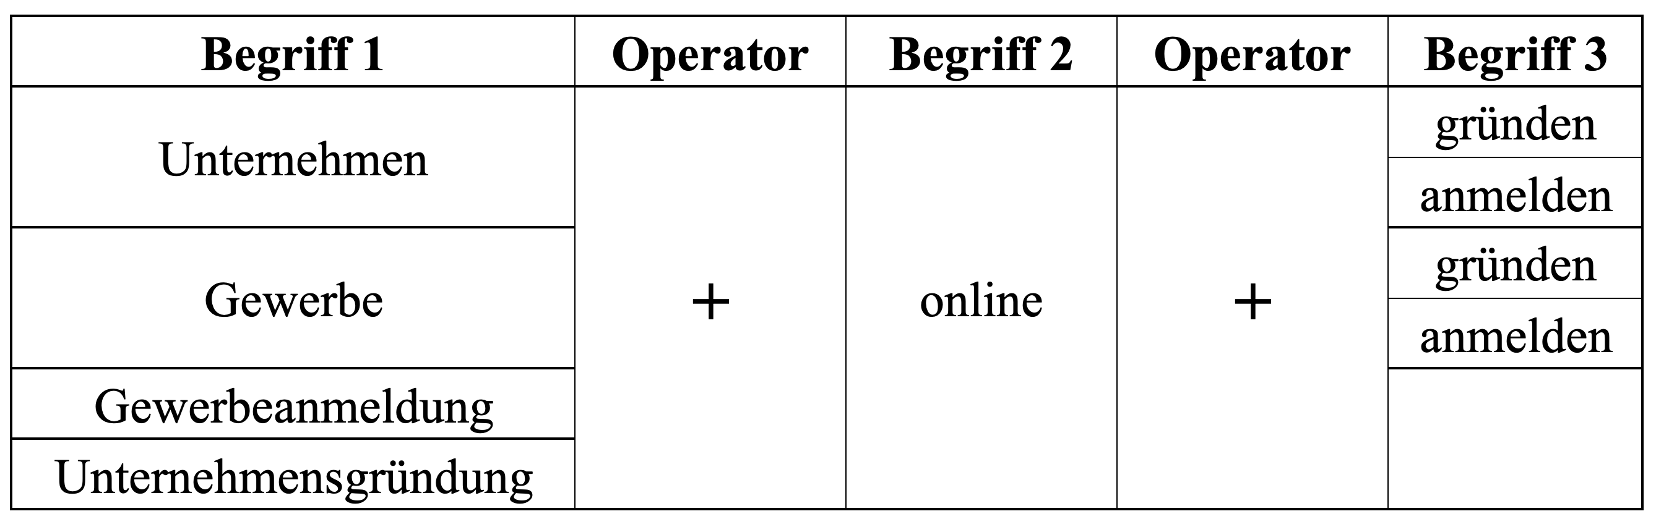
\includegraphics[width=1\textwidth]{Tabelle 1.png}
    \centering
    \caption{Suchbegriffe für die Wettbewerbsanalyse, Quelle: Eigene Darstellung}
	\label{fig:tabelle1}
\end{table}

Zum Zeitpunkt der Recherche im Januar 2025 konnte kein Anbieter gefunden werden, der eine vollumfassende Unternehmensgründung mit Anmeldung beim Gewerbeamt, Finanzamt, der Prüfung des Unternehmensnamens und einer Eintragung in das Handelsregister anbietet. Allerdings wurden einige Dienstleister gefunden, die bei der Unternehmensgründung unterstützen und einige Teile des Prozesses übernehmen. Die Tabelle 2 gibt einen Überblick über die kommerziellen Anbieter und deren Dienstleistungen, staatliche Institutionen und Behörden wurden nicht berücksichtigt. Bei der Recherche wurden als Bewertungskriterien die Gesellschaftsformen Einzelunternehmen, Gesellschaft mit beschränkter Haftung (GmbH), Gesellschaft bürgerlichen Rechts (GbR), Unternehmensgesellschaft (UG), Aktiengesellschaft (AG) herangezogen.

\begin{table}[H]
    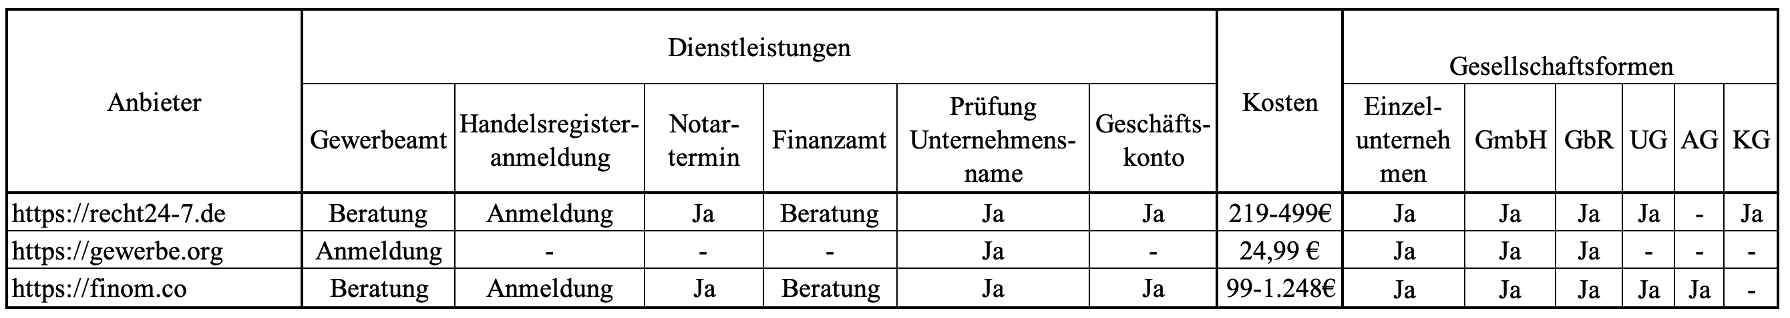
\includegraphics[width=1\textwidth]{Tabelle 2.png}
    \centering
    \caption{Ergebnisse der Wettbewerbsanalyse, Quelle: Eigene Darstellung}
	\label{fig:tabelle2}
\end{table}

Der erste Anbieter, „recht24-7.de“, berät die Kunden zur Anmeldung beim Gewerbeamt und Finanzamt. Die Leistungen umfassen außerdem die Vereinbarung eines Notartermins sowie die Prüfung des Unternehmensnamens und die Anmeldung beim Handelsregister. Auch die Eröffnung eines Geschäftskontos ist in den Leistungen des Anbieters enthalten. Die Kosten des Services liegen je nach Gesellschaftsform zwischen 219 und 499 € und es können eine Vielzahl von Gesellschaftsformen angemeldet werden. \vglfootcite[]{oa_gmbh_nodate}
Der zweiten Anbieter, „gewerbe.org“, bietet lediglich die Beratung und Anmeldung des Gewerbes beim Gewerbeamt an und es können lediglich Einzelunternehmen, Gesellschaften mit beschränkter Haftung (GmbH) sowie Gesellschaften bürgerlichen Rechts (GbR) angemeldet werden. Der Service Kostet 24.99 € (Stand Januar 2025). \vglfootcite[]{oa_unternehmen_nodate}
Der Anbieter „finom.co“ bietet ähnliche Leistungen wie „recht24-7.de“ an. Es werden also die Anmeldung beim Handelsregister sowie die Prüfung des Unternehmensnamens und die Einrichtung übernommen und ein Termin beim Notar vereinbart. Außerdem werden die Gründer hinsichtlich der Anmeldung beim Gewerbeamt und Finanzamt beraten. Auch auf „finom.co“ lassen sich zahlreiche Gesellschaftsformen Gründen unter anderem auch Aktiengesellschaften (AG). Die Kosten des Services sind abhängig von der Gesellschaftsform und liegen zwischen 99€ und 1.248€. \vglfootcite[]{oa_finom_nodate}
Als Fazit ist zu sagen, dass zwei der gefundenen Anbieter ein umfangreiches Gesamtpaket anbieten, allerdings die Anmeldung beim Gewerbeamt und Finanzamt nicht übernehmen und darüber hinaus auch keine Möglichkeit zur Markeneintragung anbieten. Einzig der Anbieter „gewerbe.org“ bietet die Anmeldung beim Gewerbeamt an, allerdings übernimmt dieser keine weiteren Services. Somit konnte das Team im Januar 2025 keinen Anbieter in Deutschland identifizieren, der einen allumfassenden Online-Service zur Unternehmensgründung anbietet. 

\newpage

\section{Methodik} \label{methodik}
In diesem Kapitel wird auf die von diesem Team angewendete Methodik zur Findung einer innovativen Lösung eingegangen. Hierbei handelt es sich um den Design Thinking Prozess.

\subsection{Design Thinking Prozess} \label{designThinking}
Der Design Thinking Prozess ist eine systematische Innovationsmethode, bestehend aus fünf Phasen. Der Fokus des Design Thinking Prozess liegt dabei auf den Bedürfnissen des Menschen. Entsprechend dieser Bedürfnisse sollen die Lösungen darüber hinaus möglichst innovativ und technisch machbar sein\vglfootcite[S. 5 ff.]{vetterli_innovationsmethode_2012}.
Zu Beginn definiert das Design Team die Problemstellung und versucht darüber hinaus das gegebene Umfeld rund um das Problem, sowie wichtige Einflussfaktoren zu erfassen und zu verstehen. Dies ist die Phase des Verstehens.
Im zweiten Schritt folgt die Definitionsphase. In dieser Phase werden die Kundenbedürfnisse analysiert und erfasst. Dies kann durch direkte Kundenansprache, Visualisierungen oder durch Beobachtungen im Gesamtkontext realisiert werden.
Danach folgt der dritte Schritt, die sogenannte Entwurfsphase. In diesem dritten Schrtitt werden konkrete Lösungsvorschläge über einen kreativen Prozesse, wie zum Beispiel Brainstorming, erstellt. Hier kann jedes Gruppenmitglied uneingeschränkt eigene Lösungsvorschläge einbringen.
In Schritt vier folgt das Prototyping. Hierbei werden die in Schritt 3 gesammelten Ideen in anfassbare Prototypen umgesetzt. Die Abstraktionsstufen dieser Prototypen kann je nach Projektphase entsprechend variieren.
Im fünften und letzten Schritt des Design Thinking Prozesses erfolgt das Testing. Die zuvor erstellten Prototypen werden von realen Nutzern getestet, wobei Fehler ganz bewusst erlaubt und sogar gewünscht sind. Diese Fehler können aufgenommen, daraus gelernt und der Prototyp verbessert werden. 
Die einzelnen Phasen, können jederzeit mehrfach durchlaufen werden, um Stück für Stück die Lösung des Problems zu optimieren. Im Idealfall setzen sich die Mitglieder des Design Thinking Prozesses aus verschiedenen Fachrichtungen zusammen, um unterschiedliche Perspektiven auf die Problemstellung einzubringen. Gleichzeitig werden Prototypen möglichst schnell erstellt, um früh erste Lösungsansätze testen zu können. Radikale und ungewöhnliche Lösungsansätze sind während des gesamten Prozesses ebenfalls gewünscht\vglfootcite[S. 8 ff.]{vetterli_innovationsmethode_2012}.
In den Folgenden Unterkapiteln gehen wir auf unsere Umsetzung der einzelnen Phasen ein.
\subsubsection{Verstehen} \label{verstehen}
Die Gründung von Unternehmen und im weiteren Sinne das Anmelden eines Markenrechts in Deutschland, ist auch über mögliche Online-Kanäle ein nicht unerheblich aufwendiger Prozess\vglfootcite[]{oa_firma_nodate}.
Gleichzeitig ist die bürokratische und verwaltungstechnische Belastung der Unternehmen enorm und weiterhin steigend. Daran anschließend ist auch die fehlende Digitalisierung im Bereich der Verwaltung innerhalb von Deutschland eine weitere Hürde, die bei der Gründung eines Unternehmens hinzu kommt\vglfootcite[S. 13 ff.]{wohlrabe_burokratie_2024}.
In diesem Kontext ist uns aufgefallen, dass der ohnehin schon komplizierte Gründungsprozess, nicht einfach und schnell bewältigt werden kann – schon gar nicht digital. Zwar gibt es die Möglichkeit gewisse Behördengänge digital zu bewältigen, der Gesamtprozess bleibt dabei aber in viele Teilschritte zerstückelt, undurchsichtig und aufwendig.
Einige Mitglieder unserer Gruppe sind bisher kaum oder gar nicht in Berührung mit der Gründung von Existenzen gekommen und schrecken schon allein auf Grund des hohen Verwaltungsaufwands vor der Gründung eines Unternehmens zurück. Andere wiederum haben schon eigene Unternehmen gegründet und können den komplizierten und kaum digital zu bewältigenden Verwaltungsaufwand bestätigen.
Im anzuwendenen Beispiel der RFInnotrade, ist es aus sicht des Gründers, welcher im Laufe des design thinking Prozesses auch als Kunde dargestellt wird, ein erheblicher Aufwand und gleichzeitg ein großer einschränkender Faktor bei der Skalierung des eigenen Unternehmens. Gute Ideen können nicht schnell und einfach umgesetzt werden, sodass diese im Zweifel sogar verloren gehen.
Zwar spielen für den Erfolg der Idee auch andere Faktoren wie Geld und in erster Linie die Qualität des Produkts eine Rolle, jedoch sollte das Scheitern an den Gründungsprozessen nicht die finale Hürde darstellen.
Es fehlt also eine konkrete und anwendbare Möglichkeit, die Unternehmensgründung einfach, automatisch und möglichst digital umzusetzen. Dadurch fehlt es auch der RFInnotrade während der Gründung von weiteren Subunternehmen, Marken und Submarken, an einer einfachen Dokumentation und Verwaltungsmöglichkeit der laufenden Gründungsprozesse.
\subsubsection{Definieren} \label{definieren}
Der Trend geht aktuell dahin, eigene Ideen möglichst schnell und einfach umzusetzen und zum Beispiel in Form eines Start-Ups an den Markt zu gehen. Dieser Schritt erscheint auf Grund der in der ersten Phase analysierten Probleme als große Hürde. In diesem Kontext haben wir, in Form einer Mindmap und über mehrere Sessions hinweg, konkrete Kundenbedürfnisse zusammengetragen.
Ein Bedürfnis der Kunden ist nach unserer Analyse, ein einfacher Überblick über alle für den Gründungsprozess notwendigen prozessualen Schritte. Dazu gehört auch der Prozess der Umfirmierung eines bereits bestehenden Unternehmens.
Ein weiteres Bedürfnis der Kunden ist die Möglichkeit, den gesamten Prozess digital und aus einer Hand heraus abzuwickeln. Gemeint ist damit der Wunsch nach einer Umsetzung über eine einzige Anlaufstelle, da zurzeit viele verschiedene Instanzen einzeln und nacheinander aufgesucht werden müssen. Außerdem sollen Anträge und Genehmigungsverfahren, möglicht schnell abgewickelt werden können. Damit verbunden ist auch eine Reduzierung der Rückfragen auf Grund fehlender oder falsch eingereichter Unterlagen.
Im Kontext der Digitalisierung ist es auch notwendig, die personenbezogene Identifizierung vollständig digital durchführen zu können. Ebenfalls sollte es digital möglich sein, den aktuellen Status der Anträge und Genehmigungsverfahren abfragen zu können und die Bezahlung des Gesamtvorgangs digital abwickeln zu können.
Als weiteres Bedürfnis haben wir die Unterstützung bei der Auswahl zur passenden Rechtsform und bei der rechtlichen Recherche zur Anmeldung einer Marke ausgemacht.
In einer späteren Wiederholung dieser Phase wurde nochmals hervorgehoben, dass es am Ende möglichst wenige oder nur ein Klick bis zum Ziel sein soll. Danach sollen sich die Funktionen des Portals ausrichten.
\subsubsection{Ideenfindung} \label{ideenfindung}
In diesem Schritt wollten wir unsere verschiedenen Ideen in Form eines Brainstormings sammeln, bewerten und weiterentwickeln.
Im Laufe des Brainstormings ist allerdings recht schnell klar geworden, dass wir uns alle auf eine Umsetzung in Form einer Webseite fokussieren wollen und diese Variante auch als vielversprechende Möglichkeit einschätzen, da die bereits gegebene Struktur eine passende Plattform bietet.
In Folge dessen haben wir uns also mehr auf die Weiterentwicklung der Idee und Umsetzung der einzelnen Kundenbedürfnisse fokussiert und in mehreren Runden verschiedene Ideen und Aspekte eingebracht.
Das Grundkonzept besteht aus einem Portal, welches in Form einer Webseite umgesetzt wird. Ziel soll es sein, die vielen verschiedenen Anlaufstellen und Prozessschritte, zentral über das Portal zu bündeln und dabei alle genannten Kundenbedürfnisse möglichst digital umzusetzen.
Über das Portal soll der Kunde zunächst, Schritt für Schritt, an den Gründungsprozess und die damit verbundenen Teilschritte herangeführt werden. Voraussetzung ist, dass der Kunde die Idee für sein Unternehmen oder seine Marke bereits ausgearbeitet hat und nun die konkrete Gründung oder Anmeldubg in Angriff nimmt. Die notwendigen Schritte zur Unternehmensgründung sollen ihm sowohl strukturiert und ansprechend visualisiert als auch erläutert werden. Für eine Umfirmierung soll das gleiche Konzept, mit angepassten Schritten verwendet werden.
Durch die gut ausgearbeitete Dokumentation der einzelnen Schritte, soll die Qualität der Anträge so weit angehoben werden, dass diese von den verschiedenen Instanzen möglichst unkompliziert und ohne weitere Rückfragen bearbeitet werden können.
Der digitale Identifikationsvorgang kann und soll über die digitale Ausweisfunktion unmittelbar im Portal integriert oder alternativ über ein bereits bestehendes Identifikationssystem wie PostIdent vorgenommen werden können. Zur digitalen Zahlungsabwicklung soll eine Schnittstelle zur hauseigenen Bank in die Webseite integriert werden. Über diese soll dann bei Unternehmensgründung ein neues Geschäftskonto angelegt und zur Abbuchung aller Gebühren an die verschiedenen Instanzen übermittelt werden.
Die Umsetzung zur Anzeige des aktuellen Prozessstatus, soll ebenfalls über das Portal und zu den jeweiligen Teilprozessen umgesetzt werden. Der Kunde soll wissen, ob seine Steuer-ID bereits beantragt wurde, gerade vom Finanzamt erstellt wird und benachrichtigt werden, falls Unterlagen nachgereicht werden müssen. Gleiches gilt für die Kontoeröffnung oder ein Genehmigungsverfahren.
Um überhaupt erst die Anbindung an die verschiedenen Behörden sowie die weiteren Stellen und die damit schnelle und unkomplizierte Abwicklung aller Prozesse zu ermöglichen, müssen entsprechende Schnittstellen zu den jeweiligen Instanzen geschaffen werden. Die Schnittstellen müssen so gebaut werden, dass eine Kommunikation in beide Richtungen möglich ist, um den aktuellen Prozesstatus sichtbar zu machen und um Dateien übermitteln sowie Anfordern zu können.
Um den Kunden bei der Findung einer passenden Rechtsform oder bei der rechtlichen Recherche zur Anmeldung einer Marke zu unterstützen, soll eine KI-Funktion in das Portal integriert werden. Diese soll dem Kunden anhand von gezielten Fragen und Antworten, die passende Rechtsform vorschlagen und rechtliche Zweifel bei der Markenanmeldung ausräumen.
\subsubsection{Prototyping \& Testing} \label{prototypingTesting}
Im Rahmen dieser Ausarbeitung wird Schritt vier und fünf des Design Thinking Prozesses nicht bearbeitet.\\
\newpage

\section{Fazit} \label{fazit}
Fazit
%-----------------------------------
% Apendix / Anhang
%-----------------------------------
\newpage
\section*{Anhang} %Überschrift "Anhang", ohne Nummerierung
\addcontentsline{toc}{section}{Anhang} %Den Anhang ohne Nummer zum Inhaltsverzeichnis hinzufügen

\begin{appendices}
	% Nachfolgende Änderungen erfolgten aufgrund von Issue 163
	\makeatletter
	\renewcommand\@seccntformat[1]{\csname the#1\endcsname:\quad}
	\makeatother
	\addtocontents{toc}{\protect\setcounter{tocdepth}{0}} %
		\renewcommand{\thesection}{\appendixname\ \arabic{section}}
		\renewcommand{\thesubsection}{\appendixname\ \arabic{section}.\arabic{subsection}}
		\renewcommand{\appendixtocname}{Anhang}
		% \section{Literaturanhänge}
% Hier werden die Literaturanhänge eingefügt, wie z.B. Snapshots der Internetseiten, die für die Recherche verwendet wurden.
% Zusammen mit der Seminararbeit wurden folgende Anhänge eingereicht:

% \begin{itemize}
%     \item besten-react-tutorials
% \end{itemize}

% \section{GitHub Repositories}
% Here are the links to the GitHub repositories that contain the code and data from the \LaTeX Project used in this paper:
% \begin{itemize}
%     \item \href{https://github.com/nilsrueber/ITInfraPaper}{ITInfraPaper}
%     \item \href{https://github.com/Foxx-l/WASMvsJS}{WASMvsJS}
% \end{itemize}
	\end{appendices}
	\addtocontents{toc}{\protect\setcounter{tocdepth}{2}}

%-----------------------------------
% Literaturverzeichnis
%-----------------------------------
\newpage

% Die folgende Zeile trägt ALLE Werke aus literatur.bib in das
% Literaturverzeichnis ein, egal ob sie zietiert wurden oder nicht.
% Der Befehl ist also nur zum Test der Skripte sinnvoll und muss bei echten
% Arbeiten entfernt werden.
%\nocite{*}

%\addcontentsline{toc}{section}{Literatur}

% Die folgenden beiden Befehle würden ab dem Literaturverzeichnis wieder eine
% römische Seitennummerierung nutzen.
% Das ist nach dem Leitfaden nicht zu tun. Dort steht nur dass 'sämtliche
% Verzeichnisse VOR dem Textteil' römisch zu nummerieren sind. (vgl. S. 3)
%\pagenumbering{Roman} %Zähler wieder römisch ausgeben
%\setcounter{page}{4}  %Zähler manuell hochsetzen

% Ausgabe des Literaturverzeichnisses

% Keine Trennung der Werke im Literaturverzeichnis nach ihrer Art
% (Online/nicht-Online)
%\begin{RaggedRight}
%\printbibliography
%\end{RaggedRight}

% Alternative Darstellung, die laut Leitfaden genutzt werden sollte.
% Dazu die Zeilen auskommentieren und folgenden code verwenden:

% Literaturverzeichnis getrennt nach Nicht-Online-Werken und Online-Werken
% (Internetquellen).
% Die Option nottype=online nimmt alles, was kein Online-Werk ist.
% Die Option heading=bibintoc sorgt dafür, dass das Literaturverzeichnis im
% Inhaltsverzeichnis steht.
% Es ist übrigens auch möglich mehrere type- bzw. nottype-Optionen anzugeben, um
% noch weitere Arten von Zusammenfassungen eines Literaturverzeichnisse zu
% erzeugen.
% Beispiel: [type=book,type=article]
\printbibliography[nottype=online,heading=bibintoc,title={Quellenverzeichnis}]

% neue Seite für Internetquellen-Verzeichnis
% brauchen wir nur wenn wir die Qellen getrennt ausgeben wollen
\newpage

% Laut Leitfaden 2018, S. 14, Fussnote 44 stehen die Internetquellen NICHT im
% Inhaltsverzeichnis, sondern gehören zum Literaturverzeichnis.
% Die Option heading=bibintoc würde die Internetquelle als eigenen Eintrag im
% Inhaltsverzeicnis anzeigen.
%\printbibliography[type=online,heading=bibintoc,title={\headingNameInternetSources}]
\printbibliography[type=online,heading=subbibliography,title={\headingNameInternetSources}]

\newpage
\pagenumbering{gobble} % Keine Seitenzahlen mehr

%-----------------------------------
% Ehrenwörtliche Erklärung
%-----------------------------------
\section*{Eigenständigkeitserklärung}

\noindent Hiermit versichere ich, dass ich die angemeldete Prüfungsleistung in allen Teilen eigen\-ständig ohne Hilfe von Dritten anfertigen und keine anderen als die in der Prüfungsleis\-tung angegebenen Quellen und zugelassenen Hilfsmittel verwenden werde. Sämtliche wörtlichen und sinngemäßen Übernahmen inklusive KI-generierter Inhalte werde ich kenntlich machen. Diese Prüfungsleistung hat zum Zeitpunkt der Abgabe weder in glei\-cher noch in ähnlicher Form, auch nicht auszugsweise, bereits einer Prüfungsbehörde zur Prüfung vorgelegen; hiervon ausgenommen sind Prüfungsleistungen, für die in der Mo\-dulbeschreibung ausdrücklich andere Regelungen festgelegt sind. Mir ist bekannt, dass die Zuwiderhandlung gegen den Inhalt dieser Erklärung einen Täuschungsversuch dar\-stellt, der das Nichtbestehen der Prüfung zur Folge hat und daneben strafrechtlich gem. § 156 StGB verfolgt werden kann. Darüber hinaus ist mir bekannt, dass ich bei schwerwie\-gender Täuschung exmatrikuliert und mit einer Geldbuße bis zu 50.000 EUR nach der für mich gültigen Rahmenprüfungsordnung belegt werden kann. Ich erkläre mich damit ein\-verstanden, dass diese Prüfungsleistung zwecks Plagiatsprüfung auf die Server externer Anbieter hochgeladen werden darf. Die Plagiatsprüfung stellt keine Zurverfügungstellung für die Öffentlichkeit dar.

\vspace{2cm}

\noindent\begin{tabular}{@{}p{0.5\textwidth}@{}p{0.5\textwidth}@{}}
{\raggedleft Bonn, 12.01.25} & {\raggedright\rule{5cm}{0.4pt}} \\
& {\raggedright Unterschrift}
\end{tabular}


% \par\medskip
% \par\medskip

\vspace{5cm}

% \includegraphics{signatures.png}
\end{document}
